\chapter{Overview of Xen\label{cha:chapter3}}
This chapter will provide a background information on the Xen hypervisor and will describe its core components of split device model for I/O virtualization.

\section{Introduction of Xen\label{sec:xen}}
The Xen Project hypervisor is an open-source type-1 or bare-metal hypervisor, which makes it possible to run many instances of an operating system or indeed different operating systems in parallel on a single machine (or host) \cite{xen}. It is one of the most popular open-source hypervisors which can provide both para-virtualization and full virtualization solutions. It has been used for server and desktop virtualization and fueling the biggest clouds and web services in production today e.g. Amazon Web Services. 
\\
\\
Xen was developed at University of Cambridge in 2003 by Ian Pratt, a senior lecturer in the Computer Laboratory, and his PhD student Keir Fraser \cite{xen_wiki}. It was acquired by Citrix in 2007. Since April 15, 2013, Xen Project has become a Linux Foundation Collaborative Project with the following companies  contributing to and guiding the Xen Project as founding members: Amazon Web Services, AMD, Bromium, Calxeda, CA Technologies, Cisco, Citrix, Google, Intel, Oracle, Samsung and Verizon \cite{xen_news}.
\\
\\
Xen consists of three main components which work together to provide virtualization solution. These include Xen hypervisor, privileged guests called \textbf{Domain-0 or Dom0} and unprivileged guests called \textbf{Domain-U or DomU}. Xen hypervisor is a small software which directly runs on hardware and is responsible for CPU scheduling ,memory management and interrupt handling. After Xen hypervisor is booted, it launches Domain-0 guest which has direct access to all hardware and has native device drivers for performing I/O operations. Other unprivileged guests access hardware and perform I/O via Dom0. Dom0 is also responsible for launching and managing DomUs with the help of control stack called \textbf{Xen Toolstack} running on it. Figure \ref{xen_arch} shows the architecture of Xen virtual environment.
\begin{figure}[!htbp]
	\centering
	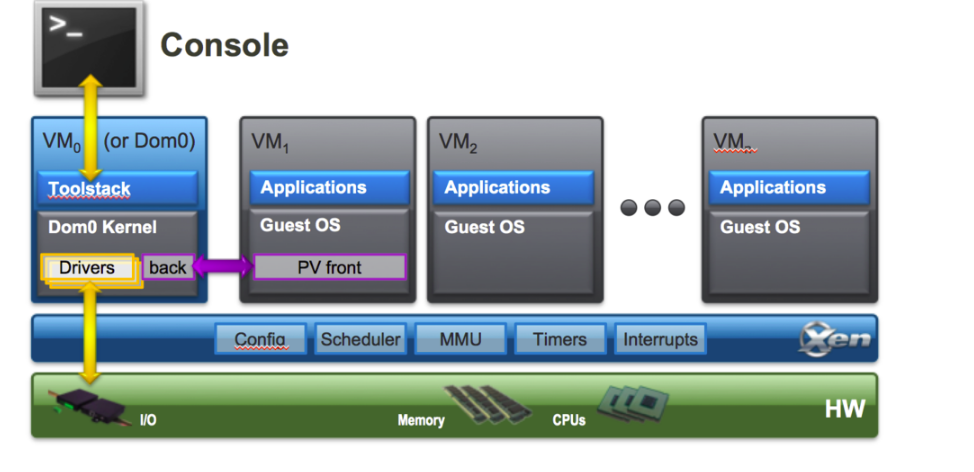
\includegraphics[width=10cm]{xen_arch}
	\caption{Basic architecture of Xen virtualization. Taken from \cite{xen_wiki}}
	\label{xen_arch}
\end{figure}
\\
\\
\subsection{Modes of Virtualization in Xen \label{sec:guests}}
Xen provides two types of virtualization modes to guests:
\begin{itemize}
	\item  \textbf{Para-virtualization (PV)}, first introduced by Xen, is a virtualization technique in which guests are modified and aware of being run on a hypervisor. A PV guest requires PV-enabled kernel with PV drivers to run on top of VMM. Dom0 in Xen is a privileged PV guest which has access to actual device drivers and hardware in the system and provides an interface to control and manage other VMs.
	\item \textbf{ Hardware-assisted or Full Virtualization (HVM)} is a virtualization mode which requires hardware virtualization extensions e.g. Intel VT or AMD-V hardware extensions support on host CPU. Guests kernels are used unmodified and hence Windows can run as HVM guest on Xen. Xen uses QEMU on HVM guests for hardware emulation and hence are slower than PV guests. However, PV drivers can be used for I/O on HVM guests to increase performance of system.
\end{itemize}

Guests having different modes virtualization can be run at the same time on Xen. It is also possible to use para-virtualization on HVM guests and vice versa. This mixing of modes introduces two other modes of virtualization on Xen which are PVHVM and PVH. In PVHVM guests, optimized PV drivers are used for disk and network virtualization on hosts with hardware support of virtualization. PVH are basically PV guests which use PV drivers for boot and I/O and use hardware virtualization for others.
\\
\\
Each mode has its pros and cons. Full virtualization provides full emulation of underlying hardware to guests which require no modifications in their OSes. However, performance is degraded while providing full emulation of entire system by VMM. Also HVM guests use trap and emulate model for execution of sensitive and privileged instructions which can cost to hundreds to thousands of cycles \cite{wang2010dynamic}. 
\\
\\
On the other hand, PV mode allows modified guests to run on a system providing an abstraction of similar physical hardware to guests and provides near native performance as compared to HVM guests. It replaces the sensitive instructions with hypercalls to VMM. It also allows combining several hypercalls into one hypercall to reduce transitions between Guests OS and VMM \cite{wang2010dynamic}.

\section{Xen on ARM I/O virtualization \label{sec:xendevice}}
Xen on ARM virtualizes CPU, memory, interrupts and timer. It does not have any knowledge of I/O devices. Access to actual physical I/O devices and their native device drivers is present in privileged Domain-0. Unprivileged guests can get access to I/O devices through Dom0. Xen assigns all I/O devices to Dom0. Dom0 is then responsible for MMIO remapping and interrupt handling. \\
\\
I/O virtualization in Xen consists of two pairs of PV drivers called \textbf{frontend and backend drivers}.For each class of hardware devices i.e. disk, network, console, framebuffer, mouse, keyboard, etc, a pair of PV drivers is present in system. 
\subsection{PV Backends and Frontends}
PV backends are implemented in Dom0 with their corresponding frontends are present in DomU. These PV drivers are implemented as kernel drivers. However, some backends can run in QEMU in userspace. Communication between frontends and backends is done through a shared memory ring protocol and events notifications mechanism provided by Xen. Xen provides tools to setup communication layer between frontend and backend drivers in Dom0 \cite{xen_arm}. Figure \ref{xen_device} shows the general I/O device virtualization architecture in Xen.
\begin{figure}[!htbp]
	\centering
	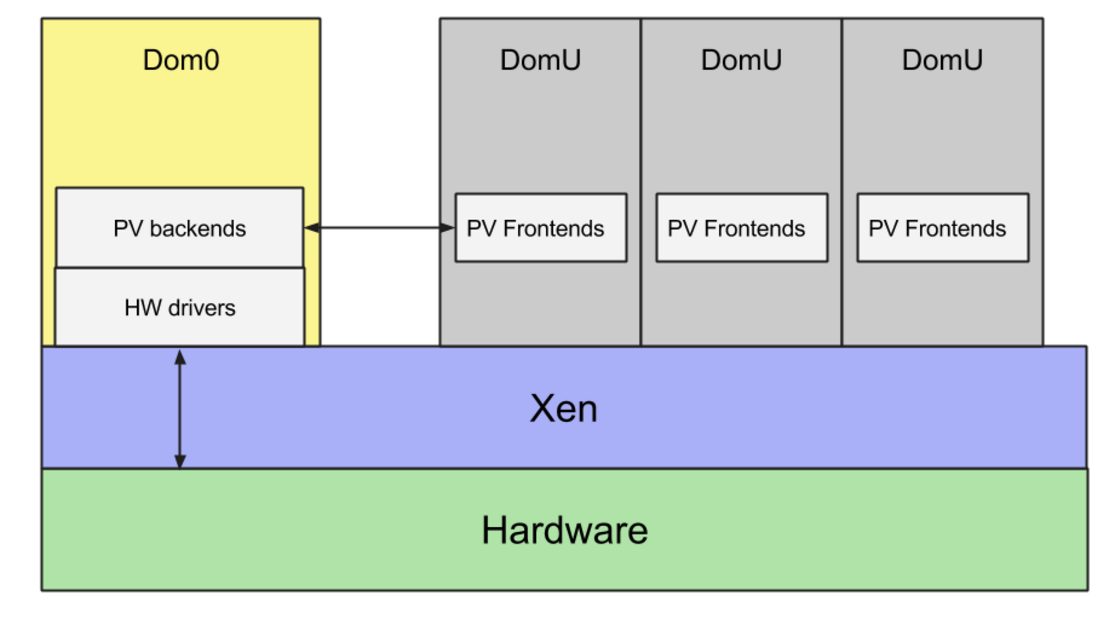
\includegraphics[width=10cm]{XEN_Device_Arch}
	\caption{Xen I/O Device Virtualization Architecture. Taken from \cite{xen_arm}}
	\label{XEN_Device_Arch}
\end{figure}

\subsection{Driver Domains}
In order to provide isolation, security and disaggregation, Xen has introduced the concept of driver domains. These are unprivileged guests running backends and native I/O drivers. Driver domain does not affect other guests or domains in case of being compromised or crashed. Figure \ref{driver_domain} shows the architecture of driver domain in Xen.

\begin{figure}[!htbp]
	\centering
	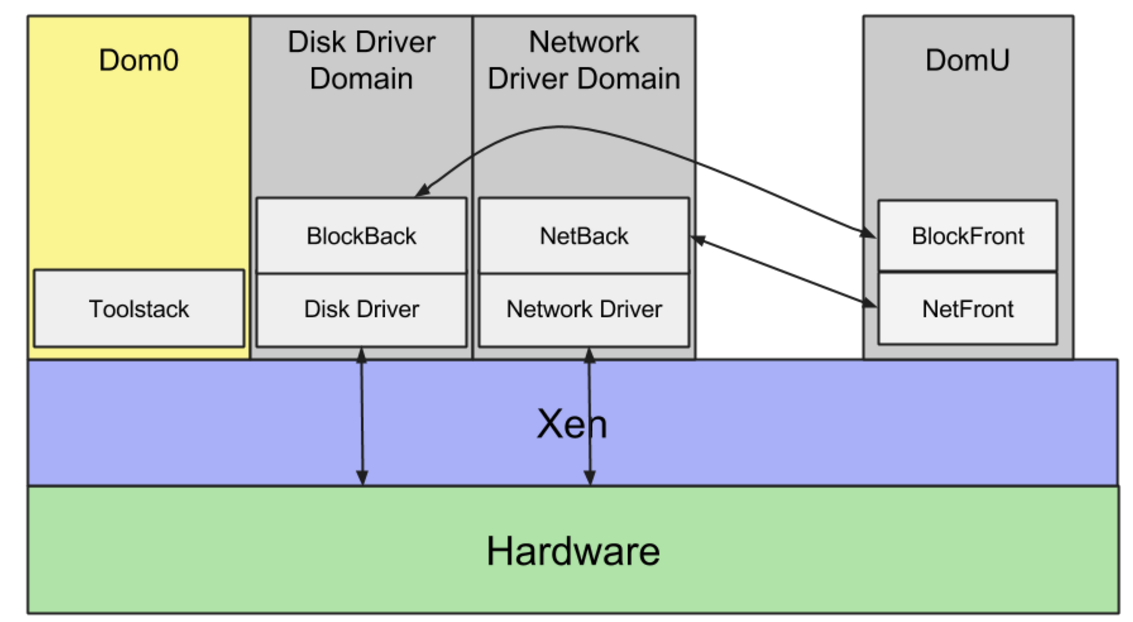
\includegraphics[width=10cm]{driver_domain}
	\caption{Xen Driver Domains Architecture. Taken from \cite{xen_arm}}
	\label{driver_domain}
\end{figure}

\subsection{Basic Features\label{sec:xendevice}}
Xen on ARM is a simple, smaller and faster as compared to its x86 counterpart. Some of its main features are described as follows:
\begin{itemize}
	\item It does not perform any emulation. There is no QEMU emulation in Xen on ARM.
	\item It exploits hardware virtualization support for memory management, interrupts and timer virtualization.
	\item It uses PV pair of drivers for I/O virtualization.
	\item It runs entirely in hypervisor mode and provides hypercalls to guest VMs for switching between hypervisor and kernel modes.
	\item It uses virtualization aware GIC for interrupt handling.
	\item It uses virtualization aware GT for timer virtualization.
	\item It supports only one type of guests which exploits hardware virtualization as much as possible and uses PV interfaces for I/O device virtualization.
\end{itemize}

Figure \ref{xen_on_arm} illustrates the simple architecture of Xen on ARM platforms.
\begin{figure}[!htbp]
	\centering
	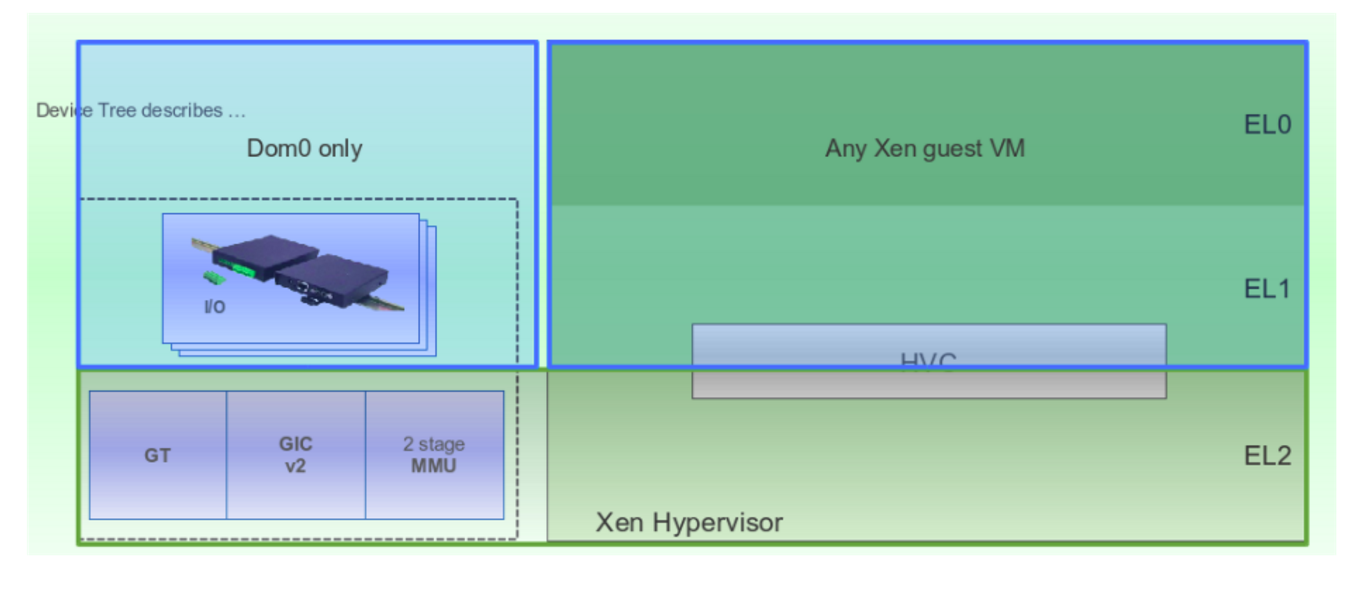
\includegraphics[width=10cm]{xen_on_arm}
	\caption{Basic architecture of Xen on ARM platforms. Taken from  \cite{xen_arm}}
	\label{xen_on_arm}
\end{figure}

\section{Xen Split I/O Driver Model\label{sec:xensplit}}
With the prevalence of embedded systems in our everyday life, enhancements in I/O devices has increased significantly. As described in previous sections, Xen delegates all I/O devices to  Dom0 or driver domains. All other guests access those I/O devices via Dom0 or driver domains. Xen uses a split driver model for multiplexing and accessing I/O devices. It supports virtualization of wide range of diverse I/O devices i.e. net, block, console, keyboard, mouse, framebuffer, XenGT(intel Graphic
card), 9pfs, PVCalls, multi-touch, sound and sisplay devices \cite{xen_release}.

\subsection{Basic Components of Xen Split I/O Driver Model\label{sec:basiccomp}}
Xen split driver model typically consists of four major components:
\begin{itemize}
	\item The native I/O device driver
	\item Top half or frontend of the split driver
	\item Bottom half or backend of the split driver
	\item Shared ring buffers
\end{itemize}

The native drivers for I/O devices are present in Dom0 or driver domains for accessing actual hardware. They are interfaced with backend drivers which provide a generic interface and I/O device multiplexing functionality. Frontend drivers are present in unprivileged guests and communicate with backends using shared ring buffers. Frontends write requests on these buffers and backends write responses which are signaled through xen event notification mechanism. Successful shared memory communication between frontends and backends depends upon Xen grant tables, event channels, Xenbus and Xenstore. These mechanisms will be explained in the later sections. Figure \ref{splitdevice} shows the basic communication mechanism of Xen split driver model.
\begin{figure}[!htbp]
	\centering
	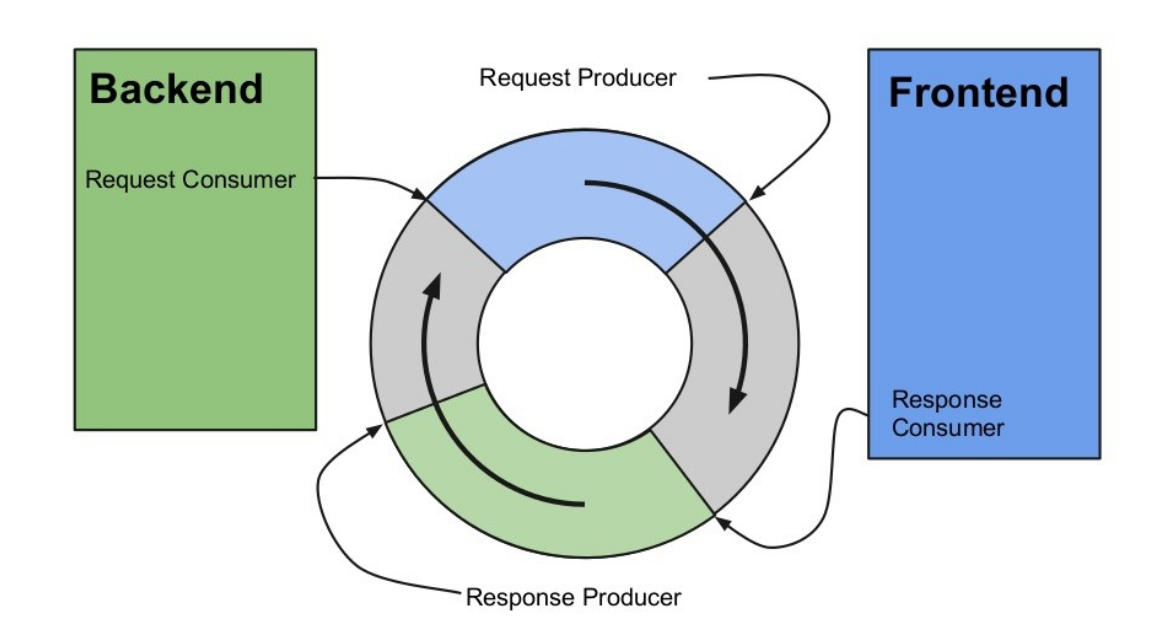
\includegraphics[width=10cm]{splitdevice}
	\caption{Communication in Xen Split Driver model. Taken from \cite{xen_slides}}
	\label{splitdevice}
\end{figure}

\subsection{Xen's Mechanisms for I/O virtualization \label{sec:basicmech}}
Xen provides following four basic mechanisms which are used by its split driver model:
\begin{itemize}
	\item Grant Tables
	\item Event Channels
    \item Xenstore
	\item XenBus Protocol
\end{itemize}
Split drivers across domains use these mechanisms to communicate with each other and access hardware devices. A brief overview for each of the above mechanisms is provided in following sections.

\subsubsection{Xen Grant Tables\label{sec:granttables}}
Grant tables is a mechanism to provide shared memory to guests. Each guests can manipulate the shared memory on page level granularity. Grant tables provides two types of operations to be performed on shared memory i.e. memory copying and memory transferring. Since Xen has access to all physical memory, it can easily copying the data between domains. Besides copying, it can also transfer a page from one domain to another by changing the page owner and modifying guests' page tables. 
\\
\\
Each guest has its grant table shared with Xen. Grant table is an array of grant entries which consist of domain ID, access flags and page frame numbers of shared pages. Each entry can be indexed using grant references which are basically integer numbers. These grant references are later placed in Xenstore ,a virtual file system for device discovery in Xen, to communicate shared page information to other domains.
\\
\\
Xen implements hypercalls for grant table operations GNTTAB\_*. Few important hypercalls are GNTTABOP\_copy, GNTTABOP\_transfer and GNTTABOP\_map\_grant\_ref. Out of these, GNTTABOP\_transfer is rarely used due to frequent TLB invalidations. It is used to transfer the ownership of page to another domain and leave the calling domain's address space. NTTABOP\_map\_grant\_ref is used to map a page into current domain's memory to allow it to perform read or write operations on it. Mapping a page removes original reference of page in sender domain's address space. GNTTABOP\_copy is the most common operation which duplicates the entire page into the local memory of calling domain. All split drivers heavily depends upon this operation.
\\
\\
Xen hypervisor creates four types of structures to implement grant mechanism:
\begin{itemize}
	\item Shared grant table is created and shared by Xen for each guest. Guest writes into entries in table and Xen performs the desired operation specified by hypercalls. Four pages are allocated and shared with each guest during initialization of each domain. A maximum of 32 pages can be allocated for shared grant tables.
	\item Active grant table is created and maintained by Xen to keep track of active grants per domain. Four pages are allocated initially for implementing active grant table per domain by Xen.
	\item Mapped track table is created and maintained by Xen per domain for each mapped page. Initially 1024 map track entries are allocated for each domain by Xen.
	\item Status grant table is created and maintained by Xen for keeping track of status of each grant per domain.
\end{itemize}
Figure \ref{granttable} shows the basic structure of shared grant table.

\begin{figure}[!htbp]
	\centering
	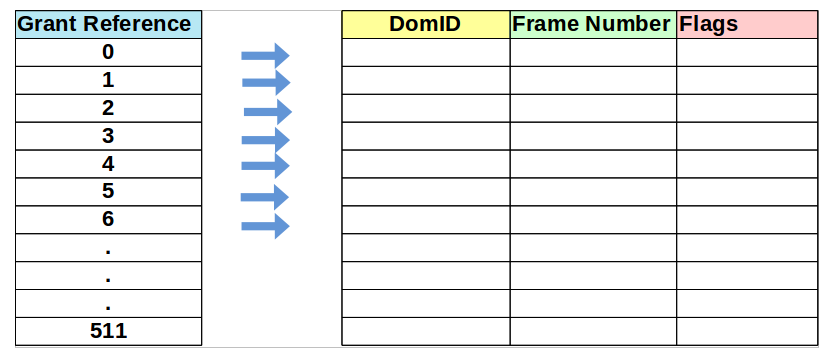
\includegraphics[width=10cm]{granttable}
	\caption{Basic structure of Shared grant table}
	\label{granttable}
\end{figure}
\textbf{Grant Table Use for Shared Ring Buffers} : 
Device I/O rings which are used for communication between split drivers are built on top this grant table mechanism. Frontend driver creates ring buffer pages and grants access to backend. Backend driver maps these shared pages for ring buffers for establishing a communication channel between domains. Figure \ref{ring} shows the actions performed by split drivers on ring buffers for inter-domain communication.

\begin{figure}[!htbp]
	\centering
	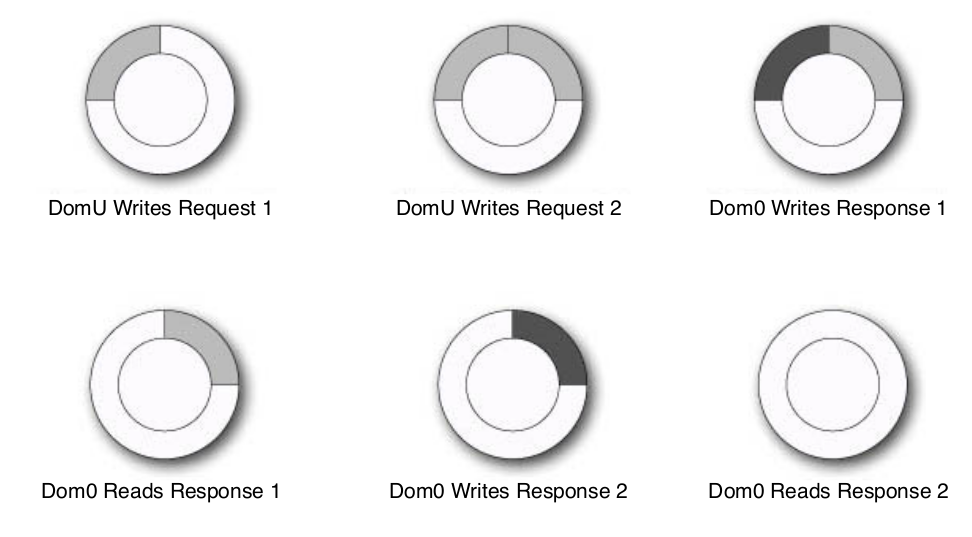
\includegraphics[width=10cm]{ring}
	\caption{Request/Response sequence on ring buffers. Taken from \cite{xen_book}}
	\label{ring}
\end{figure}

\subsubsection{Xen Event Channels\label{sec:eventchannel}}
Event channel is a mechanism for asynchronous delivery of notifications between domains. These are used with grant table mechanism to provide successful message passing between split drivers in domains. Events are similar to Unix signals. Each event represents one bit of information on which event has occured. There are four types of event channels currently supported by Xen:
\begin{itemize}
	\item Inter-domain events are used by split drivers for notifying each other about data waiting to be transported to other domain. These are bi-directional.
	\item Physical IRQ (PIRQ) are used to bind actual hardware IRQs to event channels. These are used by Domain-0 or driver domains to access various devices under their control by mapping physical IRQs to event channels.
	\item Virtual IRQs (VIRQ) are used to bind IRQs of virtual devices e.g virtual timer or emergency console to event channels.
	\item Intra-domain events are used to send events between virtual CPUs of a single domain similar to interprocessor interrupt (IPI) mechanism. These are also bi-directional similar to inter-domain events.
\end{itemize}

\textbf{Event channel creation} is a two-stage process. In the first step, an event source is bound to event channel and in second step, an event handler is registered for handling triggered event. Event channel is an abstraction of sending asynchronous notifications between domains. Each channel has two endpoints which are called ports. After binding an event channel to remote port, a domain can send an event to local port via hypercall through Xen hypervisor. Xen is then responsible for finding the remote end of channel and route events to destined remote domain.
\\
\\
\textbf{Event channel bitmap} is a structure implemented for each virtual CPU of guests running on Xen. This bitmap is shared with Xen through \textbf{`shared info'} page created during initialization of guest. When one domain sends an event to another, Xen hypervisor sets an event channel upcall pending flag and desired bit of event in destination guest's event bitmap, present in its shared info page. There are also mask bits for disabling event delivery to guests. Event delivery can be masked both by individual event type or disabling/enabling all together.
\\
\\
Xen supports two designs of implementation for event channels ABI \cite{xen_events}:
\begin{itemize}
	\item 2-level event channel ABI is de-factor implementation for event channel mechanism for which 32 bit domain supports up to 1024 event channels and 64 bit domain supports up to 4096 channels. A 2-level search path is used for finding the set event bits in event channel bitmap. For the thesis, 2-level event channel has used since 1024 events are more than enough for porting Xen's I/O split drivers to PHIDIAS.
	\item FIFO-based event channel ABI has lock-less event queues with configurable number of event channels and event priorities. It can support more thanm 100,000 event channels, with scope for 16 different event priorities.
\end{itemize}
Figure \ref{events_slide1} shows the basic structures used for 2-level event channel implementation.

\begin{figure}[!htbp]
	\centering
	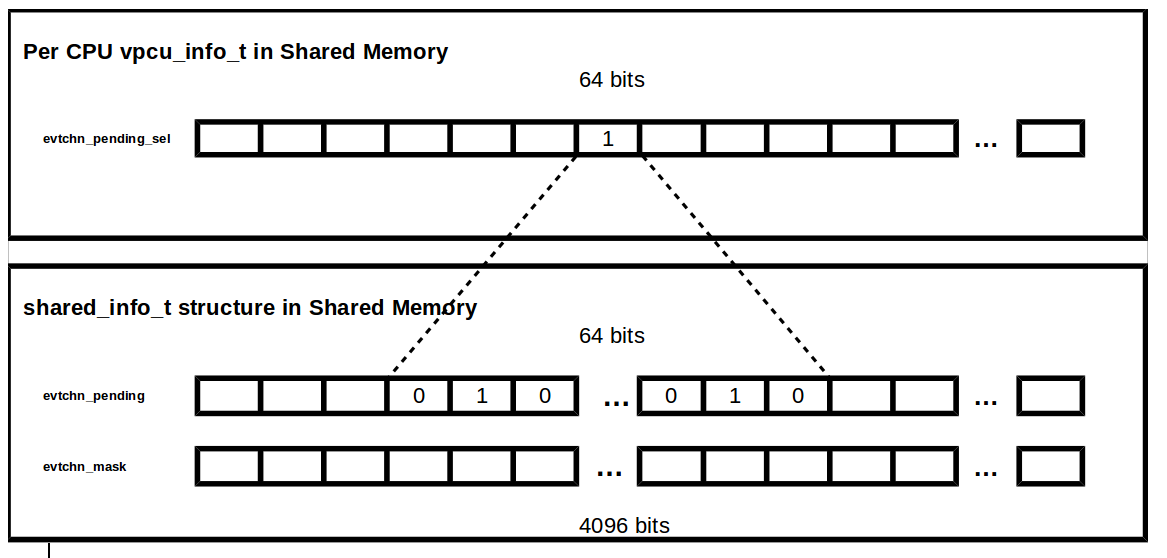
\includegraphics[width=10cm]{events_slide1}
	\caption{Bitmap of 2-level event channel ABI in Xen. Taken from \cite{events_slide}}
	\label{events_slide}
\end{figure}
\subsubsection{Xenstore \label{sec:xenstore}}
Xenstore is a hierarchical storage system maintained by Dom0 and accessed by guests through shared memory page and event channels. It is a tree database (TDB) of storage and configuration information located in Dom0. Xenstore has no hypercalls and hence can be compiled and run without depending upon Xen hypervisor. However, it needs event channels to communicate with domains using ring buffers built on top of shared memory pages. Figure \ref{xenstore} shows the basic hierarchy of Xenstore filesystem.
\begin{figure}[!htbp]
	\centering
	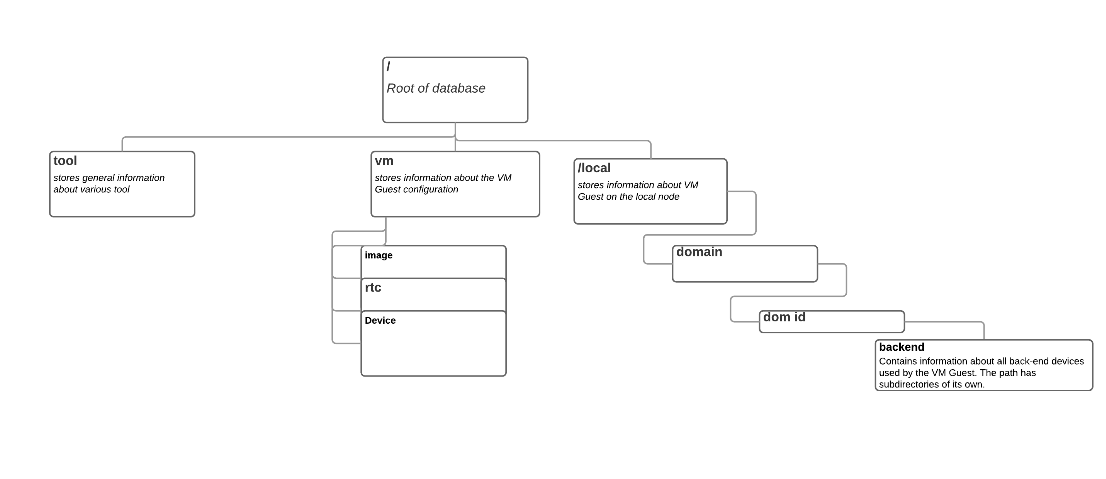
\includegraphics[width=10cm]{xenstore}
	\caption{Basic hierarchy of xenstore filesystem}
	\label{xenstore}
\end{figure}
\\
\\
There are two rings created per domain and shared with Xenstore. One for transmitting requests and other for reading responses asynchronously. Guests write requests on ring buffer and Xenstore writes responses. Only Dom0 has permissions to write or modify data stored in database of Xenstore. If DomU wants to write data in Xenstore filesystem, correct permissions must be granted to it by Dom0. Each guest shares its own memory page with Xenstore  and creates an event channel to communicate with it. Xen provides XL tool \cite{xl} to create unprivileged domains by Dom0. This tool is also responsible for registering unprivileged domains with Xenstore and map their shared memory pages into Xenstore userspace.
\\
\\
Xenstore is running as a daemon called Xenstored and allows Dom0 and guests to access information about configuration and status of the system \cite{xenstore}. Xenstore filesystem stores information in the form of directories which contains other directories or keys. Hence its structure is similar to a dictionary with key and value pairs for information. It supports handling multiple requests within a single transaction atomically to provide consistent view of stored information. The design of Xenstore interface is based on central polling loop which reads requests, polls watches and invokes callbacks \cite{xenstore_ref}.

\subsubsection{XenBus\label{sec:xenbus}} 
Xenbus \cite{Xenbus} is a protocol built on top of the XenStore used for enumerating and connecting split device drivers in Xen. Xenbus provides a bus abstraction to PV drivers to connect VM machines with each other. Its functionality depends upon grant tables, event channels and Xenstore. XenBus implements a state machine which keeps track of several states of PV drivers during the process of enumeration of virtual devices. Each split driver registers itself with XenBus which in turn calls the corresponding probe function. Frontend drivers can only be probed once related backend drivers and Xenstore are up and running.
\\
\\
The core component of Xenbus interface is state enumeration which both halves of split drivers should implement. This means that while registering with XenBus, PV drivers should provide with their own implementation of \textit{\textbf{otherend\_changed}} function which switches states of the driver and performs desired setup functions depending upon the changes in state of other end of driver. Xenbus interface provides API to split drivers to register watchers with Xenstore filesystem which gets invoked upon the changes in watched node's data. Figure \ref{xenbus} shows states of backend and frontend drivers managed by Xenbus protocol.

\begin{figure}[!htbp]
	\centering
	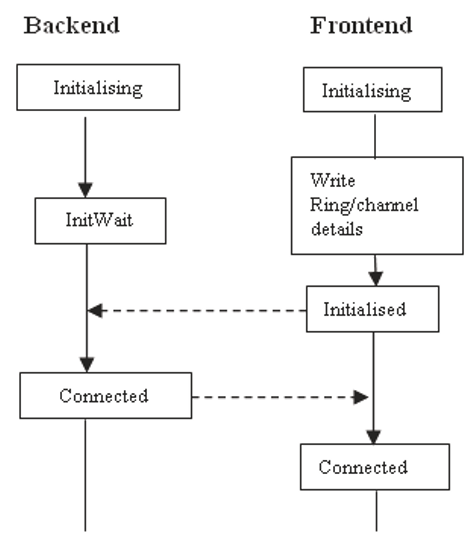
\includegraphics[width=10cm]{xenbus}
	\caption{States transition of frontend and backend drivers implemented by XenBus. Taken from \cite{cho2007sharing}}
	\label{xenbus}
\end{figure}


